\documentclass[12pt,a4paper]{article}
\usepackage[utf8]{vietnam}
\usepackage{amsmath,amssymb,amsfonts,mathrsfs}
\usepackage[left=1.5cm,right=1.5cm,top=2cm,bottom=2cm,headheight=15pt]{geometry}
\usepackage{enumitem}
\usepackage{array}
\usepackage{graphicx}
\usepackage{fancyhdr}

\pagestyle{fancy}
\fancyhf{}
\lhead{\small\textbf{HƯỚNG TỚI THPTQG 2027}}
\rhead{\small\textit{Người biên soạn: Dương Gia Bảo}}
\rfoot{\small Trang \thepage}
\renewcommand{\headrulewidth}{0.4pt}

\begin{document}

\noindent
\begin{minipage}[t]{0.40\textwidth}
    \centering
    \textbf{HƯỚNG TỚI THPTQG 2027}\\[-2pt]
    \rule{3.2cm}{0.6pt}\\[4pt]
    \textbf{ĐỀ CHÍNH THỨC}
\end{minipage}\hfill
\begin{minipage}[t]{0.58\textwidth}
    \centering
    \textbf{ĐỀ THI KHẢO SÁT CHẤT LƯỢNG}\\
    \textbf{ĐỀ SỐ 1}\\
    \textbf{Môn thi: TOÁN}\\
    \textit{\small Thời gian làm bài: 90 phút, không kể thời gian phát đề}
\end{minipage}

\vspace{0.2cm}
\noindent
\begin{minipage}[b]{0.78\textwidth}
    \textbf{Họ và tên:}\dotfill\textbf{SBD:}\makebox[3.5cm]{\dotfill}
\end{minipage}\hfill
\begin{minipage}[b]{0.20\textwidth}
    \hfill
    \setlength{\fboxrule}{0.8pt}%
    \fbox{\begin{minipage}{2.3cm}
        \centering
        \textbf{\small Mã đề thi}\\
        \textbf{0001}
    \end{minipage}}
\end{minipage}
\vspace{0.2cm}

% ==========================================
% PHẦN I
% ==========================================
\section*{\large PHẦN I. CÂU TRẮC NGHIỆM NHIỀU PHƯƠNG ÁN LỰA CHỌN}
\textit{Thí sinh trả lời từ câu 1 đến câu 12. Mỗi câu hỏi thí sinh chỉ chọn một phương án. Mỗi câu trả lời đúng được 0,25 điểm.}

\begin{enumerate}[label=\textbf{Câu \arabic*:}, leftmargin=*]

\item Cho hàm số $y = f(x)$ có bảng biến thiên như sau:
\begin{center}
\begin{tabular}{|c|ccccccc|}
\hline
$x$ & $-\infty$ & & $-1$ & & $2$ & & $+\infty$ \\ \hline
$f'(x)$ & & $+$ & $0$ & $-$ & $0$ & $+$ & \\ \hline
$f(x)$ & & $\nearrow$ & $3$ & $\searrow$ & $-1$ & $\nearrow$ & \\ 
 & $-\infty$ & & & & & & $+\infty$ \\ \hline
\end{tabular}
\end{center}
Hàm số đã cho đồng biến trên khoảng nào dưới đây?
\begin{enumerate}[label=\Alph*.]
    \item $(-1; +\infty)$.
    \item $(2; +\infty)$.
    \item $(-\infty; 2)$.
    \item $(-1; 2)$.
\end{enumerate}

\item Tập nghiệm của phương trình logarit $\log_3(2x - 1) = 2$ là
\begin{enumerate}[label=\Alph*.]
    \item $S = \left\{\dfrac{7}{2}\right\}$.
    \item $S = \{5\}$.
    \item $S = \{4\}$.
    \item $S = \{10\}$.
\end{enumerate}

\item Giá trị của tích phân $I = \int_1^3 (3x^2 - 2x) dx$ bằng
\begin{enumerate}[label=\Alph*.]
    \item $20$.
    \item $22$.
    \item $18$.
    \item $16$.
\end{enumerate}

\item Trong không gian $Oxyz$, cho hai vectơ $\vec{a} = (1; -2; 3)$ và $\vec{b} = (2; 1; -1)$. Tọa độ của vectơ $\vec{u} = \vec{a} + 2\vec{b}$ là
\begin{enumerate}[label=\Alph*.]
    \item $\vec{u} = (5; 0; 5)$.
    \item $\vec{u} = (3; -1; 2)$.
    \item $\vec{u} = (4; 0; 1)$.
    \item $\vec{u} = (5; 0; 1)$.
\end{enumerate}

\item Cho cấp số cộng $(u_n)$ có số hạng đầu $u_1 = 2$ và công sai $d = 3$. Giá trị của số hạng $u_5$ bằng
\begin{enumerate}[label=\Alph*.]
    \item $14$.
    \item $17$.
    \item $15$.
    \item $11$.
\end{enumerate}

\item Khảo sát chiều cao (đơn vị: cm) của 50 học sinh nam lớp 12 thu được mẫu số liệu ghép nhóm sau:
\begin{center}
\begin{tabular}{|c|c|c|c|c|c|}
\hline
\textbf{Chiều cao (cm)} & $[160; 165)$ & $[165; 170)$ & $[170; 175)$ & $[175; 180)$ & $[180; 185)$ \\ \hline
\textbf{Số học sinh} & $6$ & $14$ & $18$ & $8$ & $4$ \\ \hline
\end{tabular}
\end{center}
Khoảng biến thiên $R$ của mẫu số liệu ghép nhóm trên bằng
\begin{enumerate}[label=\Alph*.]
    \item $25\text{ cm}$.
    \item $15\text{ cm}$.
    \item $20\text{ cm}$.
    \item $30\text{ cm}$.
\end{enumerate}

\item Chọn ngẫu nhiên 2 học sinh từ một đội văn nghệ gồm 6 học sinh nam và 4 học sinh nữ. Xác suất để chọn được 2 học sinh đều là nữ bằng
\begin{enumerate}[label=\Alph*.]
    \item $\dfrac{2}{5}$.
    \item $\dfrac{2}{15}$.
    \item $\dfrac{1}{3}$.
    \item $\dfrac{4}{15}$.
\end{enumerate}

\item Cho hai biến cố $A$ và $B$ thỏa mãn $P(A) = 0{,}4$, $P(B) = 0{,}5$ và $P(A \cap B) = 0{,}2$. Xác suất có điều kiện $P(B|A)$ bằng
\begin{enumerate}[label=\Alph*.]
    \item $0{,}4$.
    \item $0{,}8$.
    \item $0{,}5$.
    \item $0{,}25$.
\end{enumerate}

\item Giá trị cực đại $y_{CĐ}$ của hàm số $y = x^3 - 3x + 2$ bằng
\begin{enumerate}[label=\Alph*.]
    \item $4$.
    \item $2$.
    \item $0$.
    \item $-1$.
\end{enumerate}

\item Tập nghiệm của bất phương trình mũ $2^{2x - 1} \le 8$ là
\begin{enumerate}[label=\Alph*.]
    \item $(-\infty; 1]$.
    \item $[2; +\infty)$.
    \item $(-\infty; 2)$.
    \item $(-\infty; 2]$.
\end{enumerate}

\item Trong không gian $Oxyz$, mặt phẳng đi qua điểm $M(1; 2; -3)$ và có một vectơ pháp tuyến $\vec{n} = (2; -1; 1)$ có phương trình là
\begin{enumerate}[label=\Alph*.]
    \item $x + 2y - 3z + 3 = 0$.
    \item $2x - y + z + 1 = 0$.
    \item $2x - y + z + 3 = 0$.
    \item $2x - y + z - 3 = 0$.
\end{enumerate}

\item Thể tích $V$ của khối tròn xoay thu được khi quay hình phẳng giới hạn bởi đồ thị hàm số $y = \sqrt{2x}$, trục hoành và hai đường thẳng $x = 0, x = 3$ xung quanh trục $Ox$ bằng
\begin{enumerate}[label=\Alph*.]
    \item $12\pi$.
    \item $6\pi$.
    \item $18\pi$.
    \item $9\pi$.
\end{enumerate}

\end{enumerate}

% ==========================================
% PHẦN II
% ==========================================
\section*{PHẦN II. CÂU TRẮC NGHIỆM ĐÚNG/SAI}
\textit{Thí sinh trả lời từ câu 1 đến câu 4. Trong mỗi ý a), b), c), d) ở mỗi câu, thí sinh chọn Đúng hoặc Sai.}

\begin{enumerate}[label=\textbf{Câu \arabic*:}, leftmargin=*]

\item
Một doanh nghiệp may mặc sản xuất áo khoác mùa đông. Tổng chi phí sản xuất $x$ ngàn sản phẩm ($x > 0$) được cho bởi hàm số $C(x) = x^3 - 6x^2 + 15x + 20$ (triệu đồng). Giá bán mỗi ngàn sản phẩm phụ thuộc vào số lượng sản phẩm sản xuất ra theo hàm giá $p(x) = 63 - 3x$ (triệu đồng/ngàn sản phẩm). Lợi nhuận hàng ngày của doanh nghiệp là $L(x) = R(x) - C(x) = x \cdot p(x) - C(x)$.
\begin{enumerate}[label=\alph*)]
    \item Hàm doanh thu bán $x$ ngàn sản phẩm là $R(x) = 63x - 3x^2$ (triệu đồng).
    \item Lợi nhuận của doanh nghiệp được biểu diễn bởi hàm số $L(x) = -x^3 + 3x^2 + 48x - 20$ (triệu đồng).
    \item Khi doanh nghiệp sản xuất $4$ ngàn sản phẩm thì lợi nhuận thu được là $136$ triệu đồng.
    \item Để đạt lợi nhuận lớn nhất, doanh nghiệp nên sản xuất $5$ ngàn sản phẩm (với $x$ là số nguyên) và mức lợi nhuận lớn nhất đó bằng $170$ triệu đồng.
\end{enumerate}

\item
Một đoàn tàu hỏa cao tốc đang chạy với vận tốc $v_0 = 36\text{ m/s}$ thì phát hiện chướng ngại vật từ xa và bắt đầu hãm phanh. Kể từ thời điểm bắt đầu hãm phanh $t = 0$ (giây), tàu chuyển động với gia tốc $a(t) = -0{,}8t\text{ (m/s}^2\text{)}$.
\nopagebreak[4]
\begin{center}
    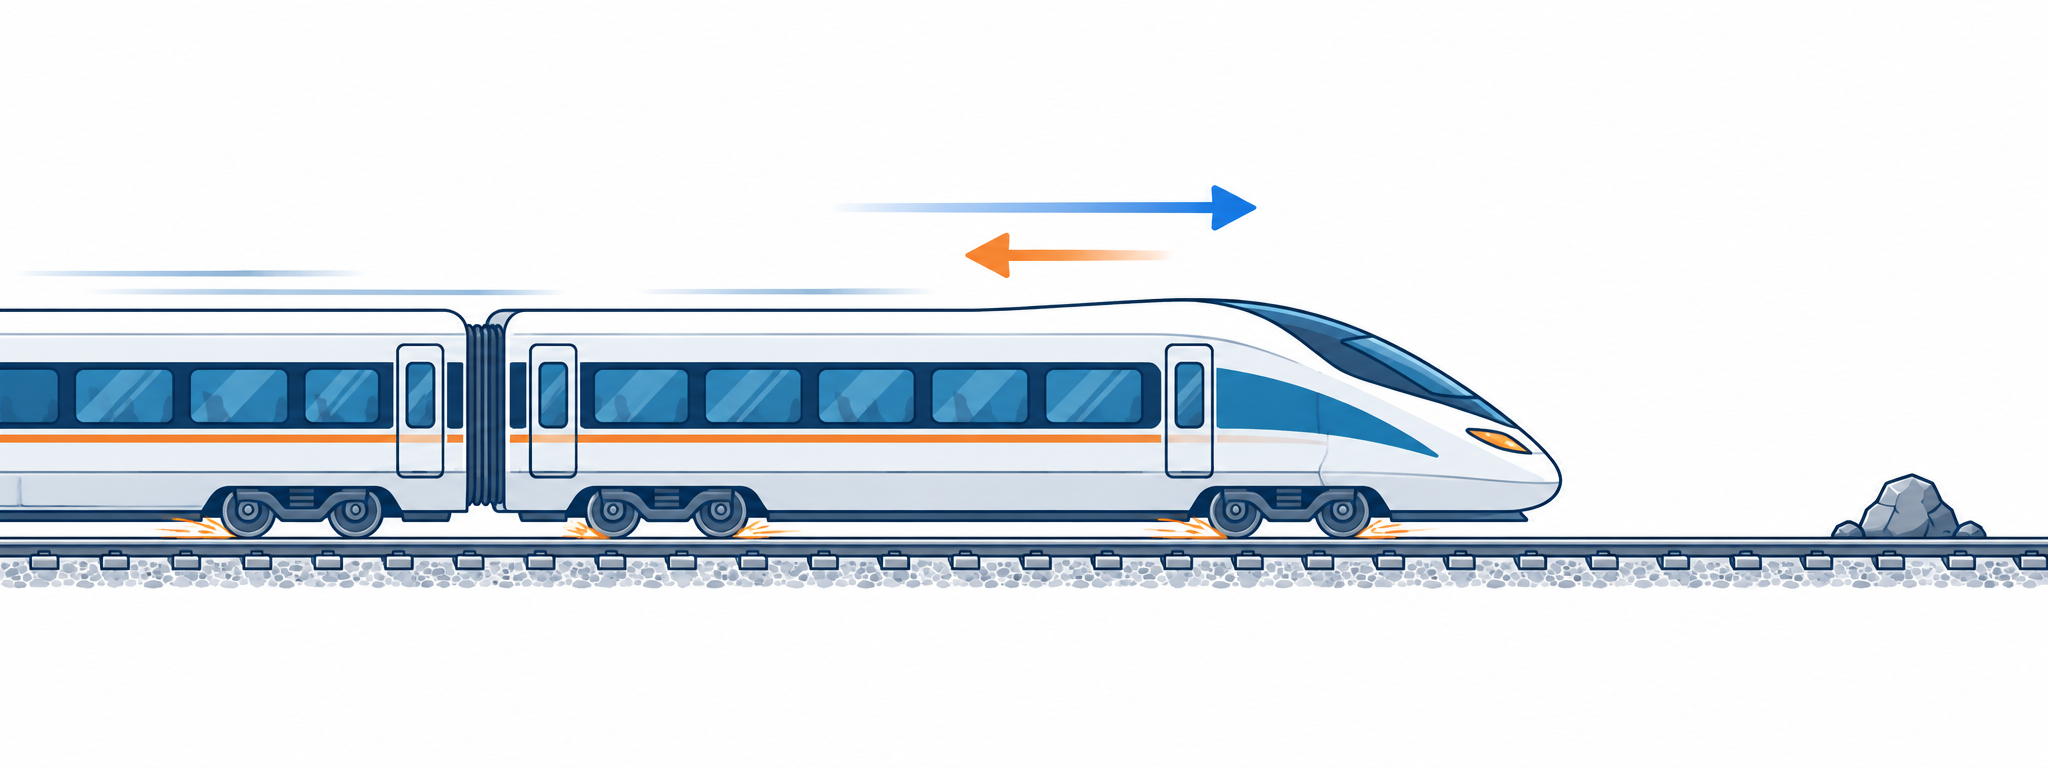
\includegraphics[width=0.62\linewidth,height=3.6cm,keepaspectratio]{images/ds-2-tau-phanh.png}
\end{center}
\nopagebreak[3]
\begin{enumerate}[label=\alph*)]
    \item Vận tốc của tàu hỏa theo thời gian $t$ là $v(t) = 36 - 0{,}4t^2\text{ (m/s)}$.
    \item Sau $5$ giây hãm phanh, vận tốc của đoàn tàu bằng $26\text{ m/s}$.
    \item Thời gian kể từ lúc bắt đầu hãm phanh cho đến khi tàu dừng hẳn là đúng $10$ giây.
    \item Tổng quãng đường đoàn tàu đi được từ lúc bắt đầu hãm phanh cho đến khi dừng hẳn vượt quá $300\text{ m}$.
\end{enumerate}

\item
Tỉ lệ người mắc bệnh tiểu đường typ 2 trong một vùng dân cư là $8\%$. Một thiết bị kiểm tra đường huyết tự động có độ nhạy $96\%$ (người mắc bệnh đo ra dương tính $96\%$) và độ đặc hiệu $92\%$ (người không mắc bệnh đo ra âm tính $92\%$). Chọn ngẫu nhiên một người trong vùng dân cư để kiểm tra. Gọi $A$ là biến cố "Người đó mắc bệnh tiểu đường" và $B$ là biến cố "Kết quả đo của người đó là dương tính".
\nopagebreak[4]
\begin{center}
    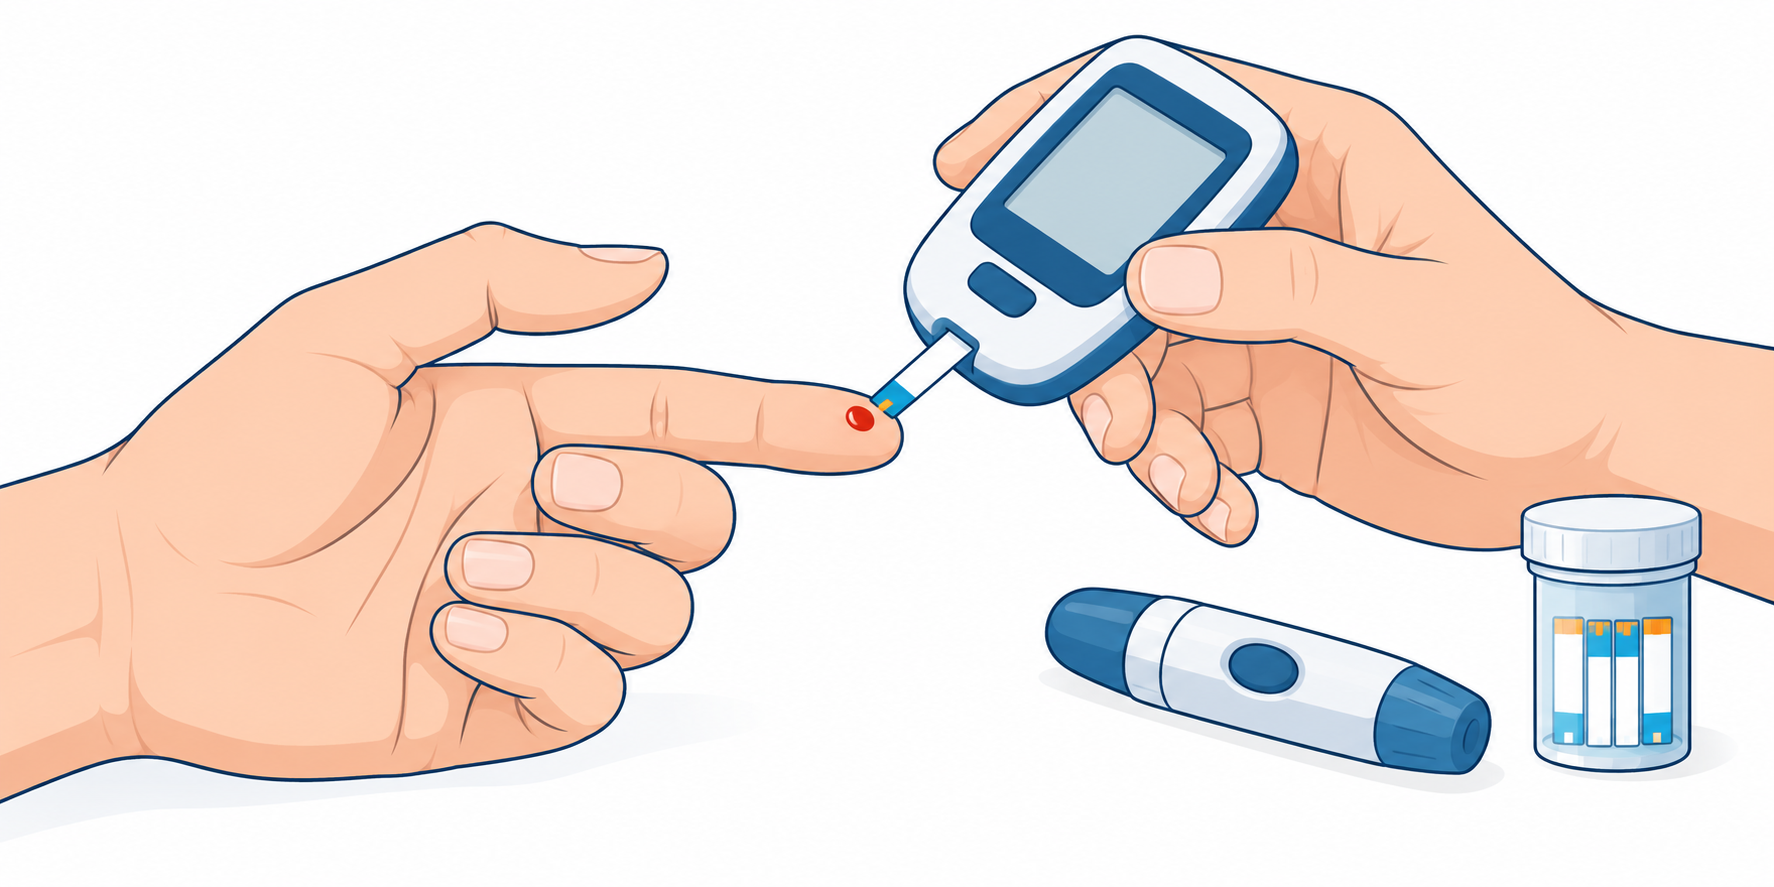
\includegraphics[width=0.62\linewidth,height=3.6cm,keepaspectratio]{images/ds-3-duong-huyet.png}
\end{center}
\nopagebreak[3]
\begin{enumerate}[label=\alph*)]
    \item Xác suất một người chọn ngẫu nhiên không mắc bệnh tiểu đường là $P(\overline{A}) = 0{,}92$.
    \item Xác suất một người không mắc bệnh tiểu đường nhưng thiết bị lại báo kết quả dương tính là $P(B|\overline{A}) = 0{,}08$.
    \item Xác suất để một người chọn ngẫu nhiên trong vùng dân cư có kết quả đo dương tính là $P(B) = 0{,}1504$.
    \item Nếu một người có kết quả đo dương tính, xác suất người đó thực sự mắc bệnh tiểu đường nhỏ hơn $50\%$.
\end{enumerate}

\item
Một khung giàn mái nhà thi đấu có dạng hình chóp $S.ABCD$ đặt trong hệ tọa độ $Oxyz$ (đơn vị trên các trục là mét). Đỉnh mái $S$ có tọa độ $S(3; 4; 6)$, các điểm góc chân mái nằm trên mặt sàn $z=0$ lần lượt là $A(0; 0; 0)$, $B(6; 0; 0)$, $C(6; 8; 0)$, $D(0; 8; 0)$. Bốn dây cáp thép chịu lực $SA, SB, SC, SD$ được chăng từ đỉnh $S$ xuống 4 góc $A, B, C, D$.
\begin{enumerate}[label=\alph*)]
    \item Tọa độ điểm $H$ là hình chiếu vuông góc của đỉnh $S$ lên mặt sàn $(ABCD)$ là $H(3; 4; 0)$.
    \item Chiều cao từ đỉnh mái $S$ đến mặt sàn $(ABCD)$ bằng $6\text{ m}$.
    \item Độ dài của cả 4 dây cáp $SA, SB, SC, SD$ đều bằng nhau và bằng $\sqrt{61}\text{ m}$.
    \item Góc tạo bởi dây cáp $SA$ và mặt sàn $(ABCD)$ nhỏ hơn $45^\circ$.
\end{enumerate}

\end{enumerate}

% ==========================================
% PHẦN III
% ==========================================
\section*{PHẦN III. CÂU TRẮC NGHIỆM TRẢ LỜI NGẮN}
\textit{Thí sinh trả lời từ câu 1 đến câu 6. Điền đáp số theo quy chuẩn làm tròn được nêu trong từng câu.}

\begin{enumerate}[label=\textbf{Câu \arabic*:}, leftmargin=*]

\item
Một cơ sở chế tác đồ trang trí tạo viên cườm đặc bằng cách quay miền bên trong elip $\dfrac{x^2}{36}+\dfrac{y^2}{16}\le 1$ quanh trục $Ox$ (đơn vị trên các trục là cm). Cơ sở khoan xuyên viên cườm một lỗ hình trụ có trục trùng với $Ox$ và bán kính không đổi. Sau khi khoan, khoảng cách giữa hai mặt phẳng vuông góc với $Ox$ đi qua hai miệng lỗ bằng $8\text{ cm}$. Tính thể tích phần vật liệu còn lại của viên cườm (đơn vị $\text{cm}^3$, làm tròn kết quả đến hàng phần mười).
\nopagebreak[4]
\begin{center}
    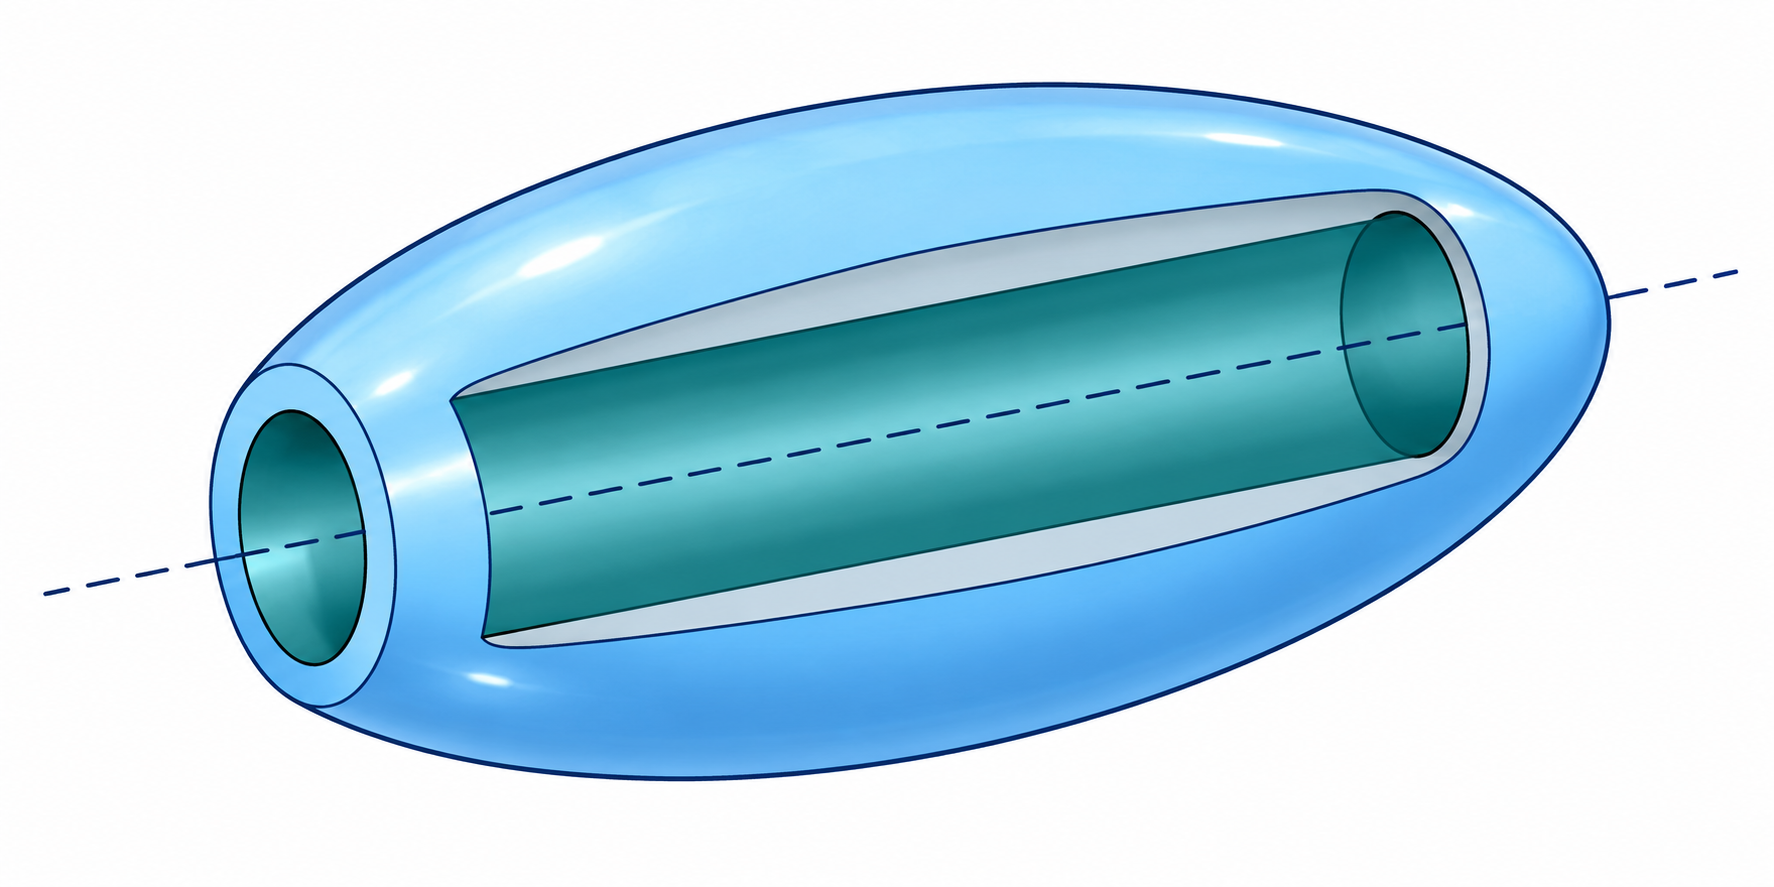
\includegraphics[width=0.62\linewidth,height=3.6cm,keepaspectratio]{images/tn-1-cuom-elip.png}
\end{center}
\nopagebreak[3]

\item
Bà Bình gửi tiết kiệm khoản tiền $500$ triệu đồng vào ngân hàng với mục đích tích lũy tài chính lâu dài cho gia đình. Ngân hàng áp dụng mức lãi suất $7\%$/năm theo hình thức lãi nhập gốc hàng năm (lãi kép). Hỏi sau ít nhất bao nhiêu năm gửi tiền thì tổng số tiền bà Bình thu được cả gốc lẫn lãi sẽ vượt quá $1$ tỷ đồng?

\item
Trong hệ tọa độ $Oxyz$ (đơn vị km), ba trạm ra-đa trên mặt đất đặt tại $A(0;0;0)$, $B(6;0;0)$ và $C(0;8;0)$. Một máy bay khảo sát bay trên mặt phẳng $(P):x-2z-2=0$; tại mọi vị trí $M$ của máy bay, khoảng cách đến hai trạm $A,B$ thỏa mãn $MA=2MB$. Máy bay có thể đi qua mọi vị trí thỏa mãn đồng thời hai điều kiện trên. Tìm khoảng cách nhỏ nhất từ máy bay đến trạm $C$ (đơn vị km, làm tròn kết quả đến hàng phần mười).
\nopagebreak[4]
\begin{center}
    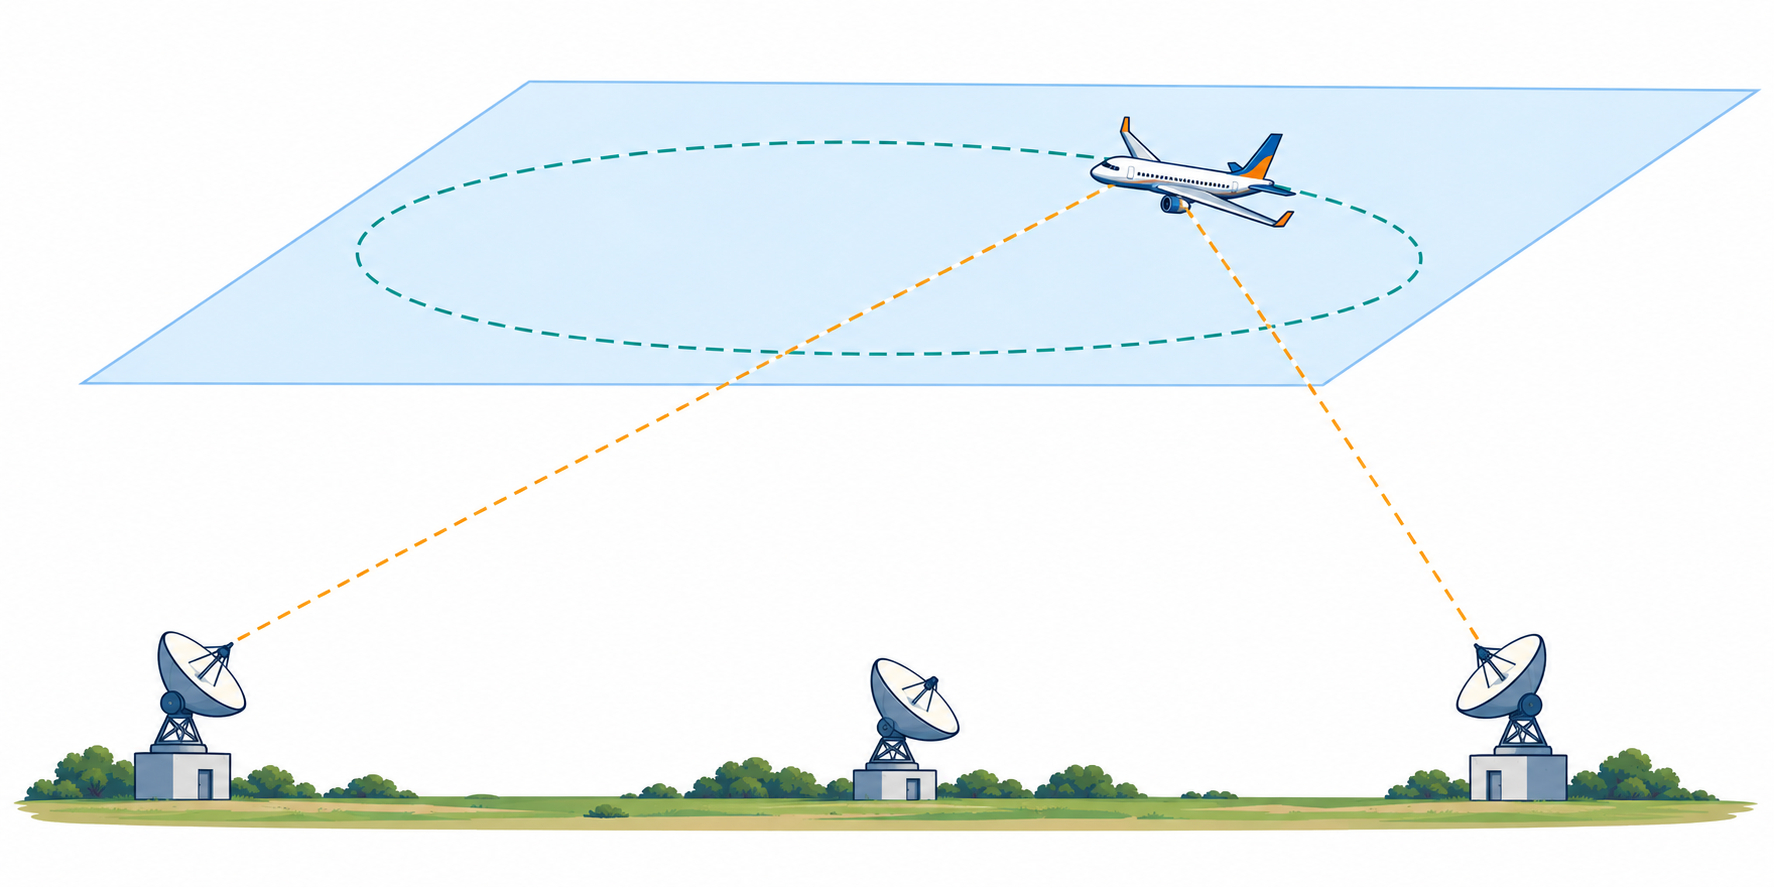
\includegraphics[width=0.62\linewidth,height=3.6cm,keepaspectratio]{images/tn-3-quy-dao-khong-gian.png}
\end{center}
\nopagebreak[3]

\item
Một kỹ sư nông nghiệp tiến hành khảo sát năng suất lúa (đơn vị: tạ/ha) tại $60$ hợp tác xã nông nghiệp vùng đồng bằng sông Hồng. Bảng số liệu ghép nhóm thu thập được như sau:
\begin{center}
\begin{tabular}{|c|c|c|c|c|c|}
\hline
\textbf{Năng suất (tạ/ha)} & $[50; 55)$ & $[55; 60)$ & $[60; 65)$ & $[65; 70)$ & $[70; 75)$ \\ \hline
\textbf{Số hợp tác xã} & $8$ & $15$ & $22$ & $10$ & $5$ \\ \hline
\end{tabular}
\end{center}
Tính tứ phân vị thứ ba $Q_3$ của mẫu số liệu ghép nhóm trên để làm căn cứ đánh giá nhóm hợp tác xã đạt năng suất cao (làm tròn kết quả đến hàng phần mười).

\item
Một xí nghiệp có ba dây chuyền sản xuất linh kiện $D_1,D_2,D_3$. Mỗi hộp hàng chứa đúng $20$ linh kiện của cùng một dây chuyền; số linh kiện hỏng trong mỗi hộp của $D_1,D_2,D_3$ lần lượt là $2,3,4$. Nhân viên chọn ngẫu nhiên một hộp, với xác suất hộp thuộc $D_1,D_2,D_3$ lần lượt là $50\%,30\%,20\%$. Từ hộp đã chọn, nhân viên lấy ngẫu nhiên đồng thời $4$ linh kiện để kiểm tra và phát hiện đúng $1$ linh kiện hỏng. Giữ riêng cả $4$ linh kiện đó, rồi lấy ngẫu nhiên đồng thời $2$ linh kiện từ $16$ linh kiện còn lại của chính hộp này. Biết kết quả lần kiểm tra đầu như trên, tính xác suất để cả $2$ linh kiện lấy lần sau đều không hỏng (làm tròn đến hàng phần mười dưới dạng $\%$, ví dụ điền $78{,}9$).
\nopagebreak[4]
\begin{center}
    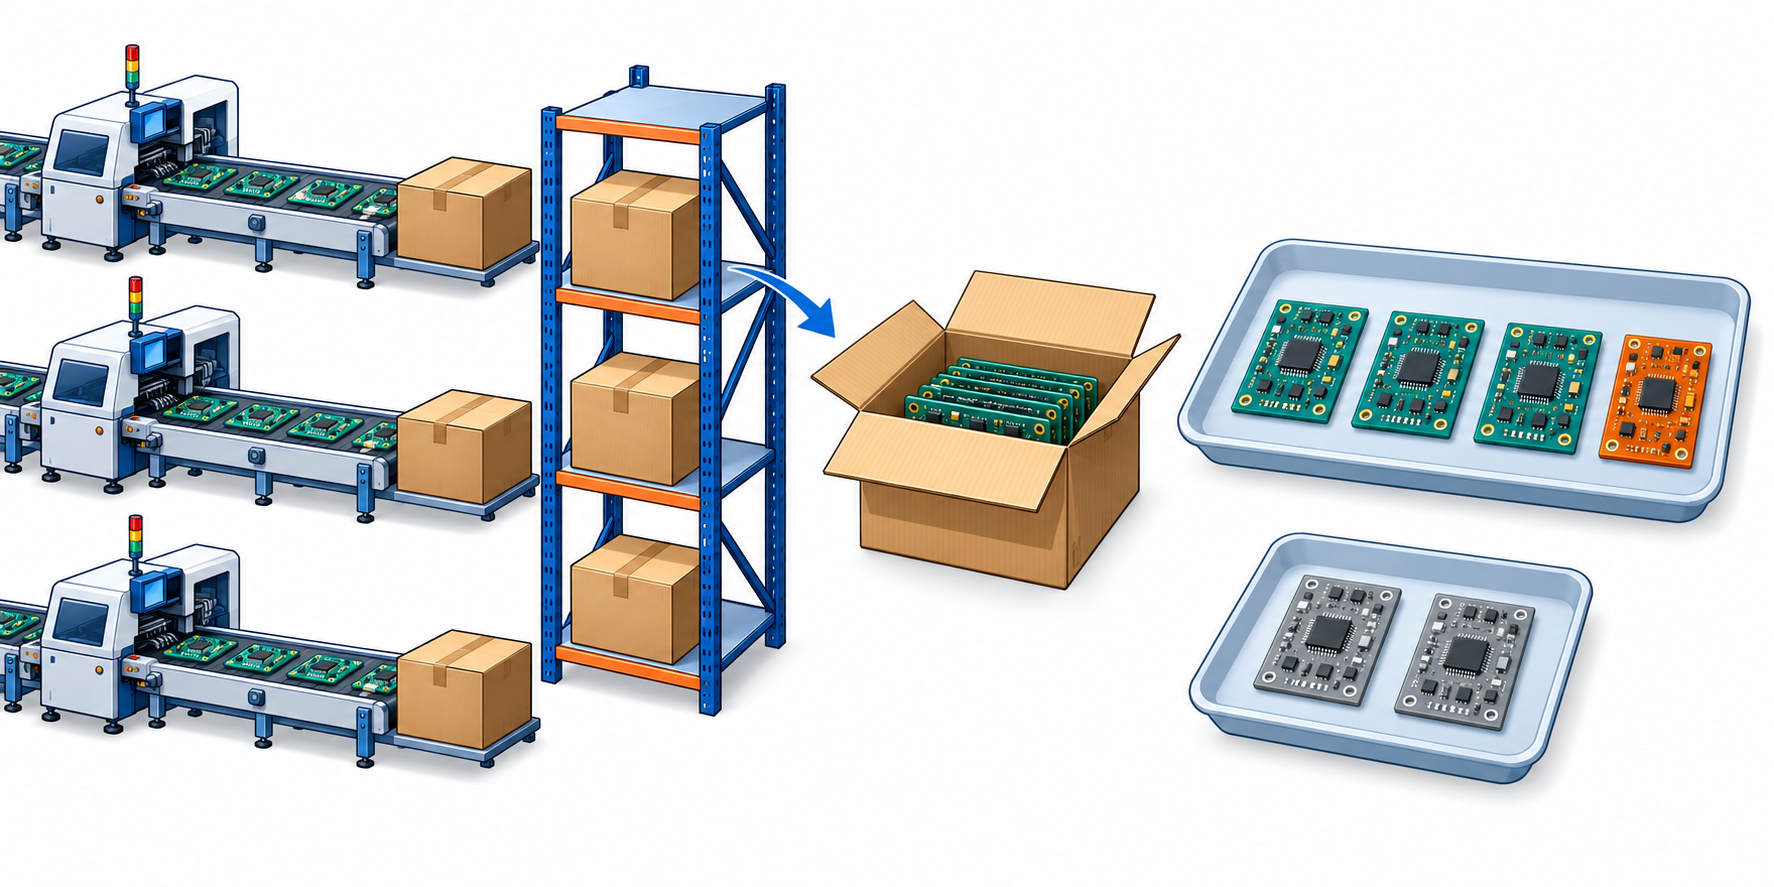
\includegraphics[width=0.62\linewidth,height=3.6cm,keepaspectratio]{images/tn-5-lay-mau-hai-dot.png}
\end{center}
\nopagebreak[3]

\item
Một đội kiểm tra an toàn thực phẩm của Sở Y tế xét nghiệm chất cấm trong các mẫu thực phẩm tại chợ đầu mối. Thực tế có $10\%$ số mẫu thực phẩm vi phạm dư lượng chất cấm. Bộ kit xét nghiệm nhanh có độ chính xác $95\%$ đối với mẫu vi phạm (dương tính thật) nhưng lại có tỉ lệ báo nhầm $5\%$ đối với mẫu an toàn (dương tính giả). Lấy ngẫu nhiên một mẫu thực phẩm để xét nghiệm. Nếu bộ kit thử báo mẫu này vi phạm (kết quả dương tính), tính xác suất để mẫu thực phẩm đó thực sự chứa chất cấm (làm tròn kết quả đến chữ số thập phân thứ nhất dưới dạng $\%$, ví dụ điền $67{,}9$).
\nopagebreak[4]
\begin{center}
    
\includegraphics[width=0.62\linewidth,height=3.6cm,keepaspectratio]{images/tn-6-kit-thuc-pham.png}
\end{center}
\nopagebreak[3]

\end{enumerate}

\newpage
% ==========================================
% BẢNG ĐÁP ÁN TỔNG HỢP
% ==========================================
\section*{BẢNG ĐÁP ÁN TỔNG HỢP}

\subsection*{1. PHẦN I}
\begin{center}
\begin{tabular}{|c|c||c|c||c|c||c|c|}
\hline
\textbf{Câu} & \textbf{Đáp án} & \textbf{Câu} & \textbf{Đáp án} & \textbf{Câu} & \textbf{Đáp án} & \textbf{Câu} & \textbf{Đáp án} \\ \hline
1 & B & 4 & D & 7 & B & 10 & D \\ \hline
2 & B & 5 & A & 8 & C & 11 & C \\ \hline
3 & C & 6 & A & 9 & A & 12 & D \\ \hline
\end{tabular}
\end{center}

\subsection*{2. PHẦN II}
\begin{center}
\begin{tabular}{|c|c|c|c|c|}
\hline
\textbf{Câu} & \textbf{Ý a)} & \textbf{Ý b)} & \textbf{Ý c)} & \textbf{Ý d)} \\ \hline
\textbf{1} & Đúng & Đúng & Sai & Đúng \\ \hline
\textbf{2} & Đúng & Đúng & Sai & Sai \\ \hline
\textbf{3} & Đúng & Đúng & Đúng & Sai \\ \hline
\textbf{4} & Đúng & Đúng & Đúng & Sai \\ \hline
\end{tabular}
\end{center}

\subsection*{3. PHẦN III}
\begin{center}
\begin{tabular}{|c|c||c|c||c|c|}
\hline
\textbf{Câu} & \textbf{Kết quả điền} & \textbf{Câu} & \textbf{Kết quả điền} & \textbf{Câu} & \textbf{Kết quả điền} \\ \hline
\textbf{1} & 119,1 & \textbf{3} & 7,8 & \textbf{5} & 78,3 \\ \hline
\textbf{2} & 11 & \textbf{4} & 65 & \textbf{6} & 67,9 \\ \hline
\end{tabular}
\end{center}

\newpage
% ==========================================
% LỜI GIẢI CHI TIẾT
% ==========================================
\section*{HƯỚNG DẪN GIẢI CHI TIẾT}

\subsection*{PHẦN I}
\begin{enumerate}[label=\textbf{Câu \arabic*:}, leftmargin=*]
\item \textbf{Đáp án B.} Nhìn vào BBT, $f'(x) > 0$ trên các khoảng $(-\infty; -1)$ và $(2; + \infty)$, do đó hàm số đồng biến trên $(2; +\infty)$.
\item \textbf{Đáp án B.} ĐKXĐ: $x > 1/2$. $\log_3(2x - 1) = 2 \iff 2x - 1 = 3^2 = 9 \iff 2x = 10 \iff x = 5$.
\item \textbf{Đáp án C.} $I = \left[x^3 - x^2\right]_1^3 = (27 - 9) - (1 - 1) = 18$.
\item \textbf{Đáp án D.} $\vec{u} = (1 + 2(2); -2 + 2(1); 3 + 2(-1)) = (5; 0; 1)$.
\item \textbf{Đáp án A.} $u_5 = u_1 + 4d = 2 + 4(3) = 14$.
\item \textbf{Đáp án A.} Khoảng biến thiên $R = x_{max} - x_{min} = 185 - 160 = 25\text{ cm}$.
\item \textbf{Đáp án B.} $P = \dfrac{C_4^2}{C_{10}^2} = \dfrac{6}{45} = \dfrac{2}{15}$.
\item \textbf{Đáp án C.} $P(B|A) = \dfrac{P(A \cap B)}{P(A)} = \dfrac{0{,}2}{0{,}4} = 0{,}5$.
\item \textbf{Đáp án A.} $y' = 3x^2 - 3 = 0 \iff x = \pm 1$. $y''(-1) = -6 < 0 \implies x = -1$ là điểm cực đại, $y_{CĐ} = y(-1) = -1 + 3 + 2 = 4$.
\item \textbf{Đáp án D.} $2^{2x - 1} \le 2^3 \iff 2x - 1 \le 3 \iff x \le 2$.
\item \textbf{Đáp án C.} $2(x - 1) - 1(y - 2) + 1(z + 3) = 0 \iff 2x - y + z + 3 = 0$.
\item \textbf{Đáp án D.} $V = \pi \int_0^3 (\sqrt{2x})^2 dx = \pi \int_0^3 2x dx = \pi \left[x^2\right]_0^3 = 9\pi$.
\end{enumerate}

\subsection*{PHẦN II}
\begin{enumerate}[label=\textbf{Câu \arabic*:}, leftmargin=*]
\item \textbf{Câu 1 (Tối ưu kinh tế):}
\begin{itemize}
    \item a) \textbf{Đúng}: $R(x) = x \cdot p(x) = x(63 - 3x) = 63x - 3x^2$.
    \item b) \textbf{Đúng}: $L(x) = R(x) - C(x) = (63x - 3x^2) - (x^3 - 6x^2 + 15x + 20) = -x^3 + 3x^2 + 48x - 20$.
    \item c) \textbf{Sai}: $L(4) = -4^3 + 3(4^2) + 48(4) - 20 = -64 + 48 + 192 - 20 = 156$ triệu đồng (không phải $136$).
    \item d) \textbf{Đúng}: $L'(x) = -3x^2 + 6x + 48 = 0 \iff x = 5{,}123$. Vì $x$ nguyên, so sánh $L(5) = 170$ và $L(6) = 160 \implies \max L = 170$ tại $x = 5$ ngàn sản phẩm.
\end{itemize}

\item \textbf{Câu 2 (Chuyển động):}
\begin{itemize}
    \item a) \textbf{Đúng}: $v(t) = 36 + \int (-0{,}8t) dt = 36 - 0{,}4t^2$.
    \item b) \textbf{Đúng}: $v(5) = 36 - 0{,}4(25) = 26\text{ m/s}$.
    \item c) \textbf{Sai}: Tàu dừng khi $v(t) = 0 \iff 36 - 0{,}4t^2 = 0 \iff t = \sqrt{90} = 3\sqrt{10} \approx 9{,}49\text{ s}$ (không phải $10\text{ s}$).
    \item d) \textbf{Sai}: $S = \left[36t - \dfrac{0{,}4t^3}{3}\right]_0^{3\sqrt{10}} = 108\sqrt{10} - 36\sqrt{10} = 72\sqrt{10} \approx 227{,}68\text{ m} < 300\text{ m}$.
\end{itemize}

\item \textbf{Câu 3 (Xác suất Bayes):}
\begin{itemize}
    \item a) \textbf{Đúng}: $P(\overline{A}) = 1 - 0{,}08 = 0{,}92$.
    \item b) \textbf{Đúng}: $P(B|\overline{A}) = 1 - 0{,}92 = 0{,}08$.
    \item c) \textbf{Đúng}: $P(B) = P(A)P(B|A) + P(\overline{A})P(B|\overline{A}) = 0{,}08 \times 0{,}96 + 0{,}92 \times 0{,}08 = 0{,}1504$.
    \item d) \textbf{Sai}: $P(A|B) = \dfrac{0{,}08 \times 0{,}96}{0{,}1504} = \dfrac{0{,}0768}{0{,}1504} \approx 51{,}06\% > 50\%$.
\end{itemize}

\item \textbf{Câu 4 (Oxyz Thực tế):}
\begin{itemize}
    \item a) \textbf{Đúng}: $S(3; 4; 6)$ chiếu lên $z=0$ là $H(3; 4; 0)$.
    \item b) \textbf{Đúng}: Khoảng cách từ $S$ đến sàn $z=0$ là $z_S = 6\text{ m}$.
    \item c) \textbf{Đúng}: $SA = \sqrt{3^2 + 4^2 + 6^2} = \sqrt{61}\text{ m}$, tương tự $SB = SC = SD = \sqrt{61}\text{ m}$.
    \item d) \textbf{Sai}: Gọi $\theta$ là góc giữa $SA$ và mặt sàn $\implies \sin\theta = \dfrac{6}{\sqrt{61}} \approx 0{,}768 \implies \theta \approx 50{,}2^\circ > 45^\circ$.
\end{itemize}

\end{enumerate}

\subsection*{PHẦN III}
\begin{enumerate}[label=\textbf{Câu \arabic*:}, leftmargin=*]
\item \textbf{Đáp số: 119,1.}
Ở vị trí có hoành độ $x$, bán kính mặt cắt ngoài thỏa mãn $R^2(x)=16\left(1-\dfrac{x^2}{36}\right)$.
Gọi $r$ là bán kính lỗ khoan. Do viên cườm và lỗ khoan đối xứng qua mặt phẳng $x=0$, hai miệng lỗ cách nhau $8\text{ cm}$ nằm tại $x=\pm4$. Tại đó, $R(4)=r$, nên
\[
 r^2=16\left(1-\frac{16}{36}\right)=\frac{80}{9}.
\]
Chỉ trên đoạn $[-4;4]$ mặt cắt còn vật liệu; diện tích mặt cắt là một vành khăn:
\[
 S(x)=\pi\bigl(R^2(x)-r^2\bigr)=\frac{4\pi}{9}(16-x^2).
\]
Vì vậy
\[
 V=\frac{4\pi}{9}\int_{-4}^{4}(16-x^2)\,dx
   =\frac{1024\pi}{27}\approx119{,}147\text{ cm}^3.
\]
Làm tròn đến hàng phần mười được $119{,}1$. Không trừ thể tích một hình trụ dài $12\text{ cm}$ khỏi toàn bộ khối elip, vì gần hai đầu viên cườm, mũi khoan lấy đi toàn bộ mặt cắt.
\item \textbf{Đáp số: 11.} $500(1 + 0{,}07)^n > 1000 \iff 1{,}07^n > 2 \iff n > \log_{1{,}07}(2) \approx 10{,}24 \implies n = 11$ năm.
\item \textbf{Đáp số: 7,8.}
Đặt $M(x;y;z)$. Điều kiện $MA=2MB$ tương đương
\[
 x^2+y^2+z^2=4\bigl((x-6)^2+y^2+z^2\bigr)
 \iff (x-8)^2+y^2+z^2=16.
\]
Như vậy $M$ thuộc giao tuyến của mặt cầu tâm $I(8;0;0)$, bán kính $4$, và mặt phẳng $(P)$. Một vectơ pháp tuyến của $(P)$ là $\vec n=(1;0;-2)$.
Hình chiếu vuông góc của $I$ lên $(P)$ là
\[
 H=I-\frac{8-2}{1^2+(-2)^2}\vec n
   =\left(\frac{34}{5};0;\frac{12}{5}\right),
 \qquad IH=\frac6{\sqrt5}.
\]
Quỹ đạo là đường tròn trong $(P)$, tâm $H$, bán kính
\[
 \rho=\sqrt{4^2-IH^2}=\sqrt{\frac{44}{5}}.
\]
Gọi $K$ là hình chiếu vuông góc của $C$ lên $(P)$. Khi đó
\[
 K=C-\frac{-2}{5}\vec n=\left(\frac25;8;-\frac45\right),
 \quad CK=\frac2{\sqrt5},\quad HK=\frac{24}{\sqrt5}>\rho.
\]
Với $M\in(P)$, $CM^2=CK^2+KM^2$. Khoảng cách $KM$ nhỏ nhất bằng $HK-\rho$, đạt được tại điểm trên đường tròn nằm trên tia $HK$. Do đó
\[
 \min CM=\sqrt{\frac45+\left(\frac{24}{\sqrt5}-\sqrt{\frac{44}{5}}\right)^2}
 =\sqrt{\frac{624-96\sqrt{11}}5}\approx7{,}818\text{ km}.
\]
Làm tròn đến hàng phần mười được $7{,}8$.
\item \textbf{Đáp số: 65.} Tứ phân vị thứ ba $Q_3$ nằm ở nhóm $[60; 65)$ với vị trí $45 \implies Q_3 = 60 + \dfrac{45 - 23}{22} \times 5 = 65{,}0$.
\item \textbf{Đáp số: 78,3.}
Gọi $E$ là biến cố lần đầu lấy được đúng một linh kiện hỏng; $F$ là biến cố lần sau lấy được hai linh kiện tốt. Đặt $d_1=2,d_2=3,d_3=4$ và $p_1=0{,}5,p_2=0{,}3,p_3=0{,}2$.
Vì lấy không hoàn lại từ một hộp, ta có
\[
 P(E\mid D_i)=\frac{d_i\binom{20-d_i}{3}}{\binom{20}{4}}.
\]
Nếu hộp thuộc $D_i$ và $E$ xảy ra, trong $16$ linh kiện còn lại có $d_i-1$ linh kiện hỏng và $17-d_i$ linh kiện tốt. Vì vậy
\[
 P(F\mid E,D_i)=\frac{\binom{17-d_i}{2}}{\binom{16}{2}}.
\]
Kết hợp xác suất toàn phần và xác suất có điều kiện:
\[
 P(F\mid E)=
 \frac{\sum_{i=1}^3p_i d_i\binom{20-d_i}{3}\binom{17-d_i}{2}}
 {\binom{16}{2}\sum_{i=1}^3p_i d_i\binom{20-d_i}{3}}.
\]
Các hệ số $d_i\binom{20-d_i}{3}$ lần lượt là $1632,2040,2240$; các hệ số $\binom{17-d_i}{2}$ lần lượt là $105,91,78$. Suy ra
\[
 P(F\mid E)=
 \frac{5\cdot1632\cdot105+3\cdot2040\cdot91+2\cdot2240\cdot78}
 {120(5\cdot1632+3\cdot2040+2\cdot2240)}
 =\frac{14693}{18760}\approx0{,}783209.
\]
Đổi sang phần trăm và làm tròn được $78{,}3\%$. Kết quả lần đầu làm thay đổi xác suất hộp thuộc từng dây chuyền, nên không dùng nguyên các trọng số ban đầu để tính xác suất lần sau.
\item \textbf{Đáp số: 67,9.} $P(A|B) = \dfrac{0{,}10 \times 0{,}95}{0{,}10 \times 0{,}95 + 0{,}90 \times 0{,}05} = \dfrac{0{,}095}{0{,}14} \approx 67{,}857\% \approx 67{,}9\%$.
\end{enumerate}

\end{document}
